\section{Methodik}
\subsection{Statische Datenerfassung}

Die statische Datenerfassung dient dem Zweck, die Funktionalität der Wandler unter einer konstanten Last zu überprüfen. Es wurden zwei simple Testfälle aufgebaut. Bei beiden handelt es sich um Parallelschaltungen von 4,7 Ohm Widerständen. Der erste Fall schaltet zwei davon parallel, der zweite drei. Durch das Anwenden des Ohmschen Gesetzes, kann ein theoretischer Stromfluss und somit auch die theoretische Leistungsaufnahme berechnet werden. Der Wandler wird durch ein Netzteil mit 24 Volt Ausgangsspannung betrieben. Diese 24 Volt werden von dem Wandler auf 12 V herabgesetzt. Somit kann der Strom berechnet werden, der durch die Widerstände fließt. Bei zwei parallel-geschaltenen Widerständen ergibt das einen theoretischen Stromfluss von 5.1 A wie und bei drei parallel geschaltenen Widerständen 7.65 A wie in den Gleichungen 3 und 4 zu sehen ist.

\begin{equation}
\label{Ohmsches Gesetz}
\frac{U}{R} = I \tab
\end{equation}


\begin{equation}
\label{Ohmsches Gesetz}
\frac{12V}{4.7 Ohm}*2 = 5.10 A 
\end{equation}


\begin{equation}
\label{Ohmsches Gesetz}
12V*4.7 Ohm*3 = 7.65 A 
\end{equation}


Da es sich in diesen Testfällen um statische Lasten handelt, sind keine hohen Abtastraten erforderlich, deshalb wird zur Datenerfassung ein PicKit mitsamt I²C Schnittstelle verwendet und kein Raspberry Pi. 

Nachdem die Daten erfasst worden sind, müssen diese noch verarbeitet werden, um die entsprechenden Werte zu erhalten.
 

\subsection{Dynamische Datenerfassung}

Das Ziel der dynamischen Datenerfassung ist es, zu evaluieren, wie der Wandler sich unter Lasten verhält, die sich mit der Zeit ändern. Sowie mögliche Abweichungen zwischen den einzelnen Wandlern selbst. Der Testaufbau beinhaltet den Hybridwandler, einen Stereoverstärker, welcher per Wandler mit Strom versorgt wird und in den ein Audiosignal eingespeist wird. In Abb. 5 ist die Schaltung des Testaufbaus abgebildet. Es ist zu erkennen, das am Eingang des Buck-Wandlers 24 V eingespeist werden und das die am Ausgang liegenden 12 V an den Stereoverstärker angeschlossen sind. Des Weiteren ist ersichtlich, dass nur ein Kanal des Stereoverstärkers genutzt wird. Dieser Kanal wird mit einem Audiosignal aus einem externen Rechner versorgt. Als Signale werden hierbei Sinussignale mit variierender Frequenz verwendet, welche mit dem Programm Audacity generiert werden (https://www.audacityteam.org/). Das Ausgangssignal fällt über einen Lastwiderstand ab. Obwohl es ein Stereoverstärker ist, wurde auf einen Lautsprecher verzichtet, da durch einen Lastwiderstand die Reproduzierbarkeit gewährleistet wird. 


\begin{figure}[H]
    \centering
    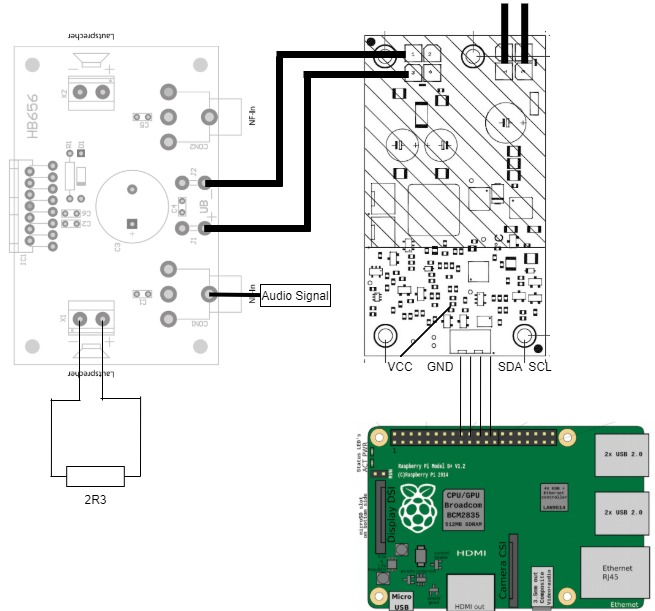
\includegraphics[height= 4cm, width = 12cm]{Pictures/Dyn_Schaltung.jpg}
    \caption{Versuchsaufbau der dynamischen Datenerfassung}
\end{figure}

Der erste Testschritt ist dabei die Überprüfung, wie hoch die maximale Frequenz eines Signals sein kann, sodass interpretierbare Daten erzeugt werden können. Die maximale Frequenz kann durch praktische Tests empirisch bestimmt werden. Der Umfang dieser Tests besteht darin, die Daten von mehreren Wandlern über einen Zeitraum T zu messen und anschließend die Anzahl der gemessenen Samples durch die gemessene Zeit zu teilen, um so die durchschnittliche Sample-Rate pro Sekunde zu erhalten. 

Dadurch, dass die Datenerfassung auf einem Raspberry Pi abläuft, ist es möglich, die Daten nach jeder Abfrage sofort in eine Textdatei abzuspeichern. Es werden Daten zur Zeit, Temperatur, Ausgangsstrom, Ausgangsspannung und Eingangsspannung aufgezeichnet und tabellarisch abgespeichert.


\begin{equation}
\label{Nyquist}
f\textsubscript{nyquist} = 1/2 * f\textsubscript{abtastrate}
\end{equation}
Die Nyquist-Frequenz stammt aus der Signaltheorie und setzt die maximale Abtastrate in Verhältnis mit der maximalen Frequenz, die ohne Verzerrungen dargestellt werden kann. Die Gleichung besagt, dass die maximale Frequenz, die ohne Verzerrungen dargestellt werden soll, mit einer Abtastrate abgetastet werden soll, die mindestens doppelt so hoch ist, wie die abgetastete Frequenz. Sobald die Abtastrate experimentell bestimmt werden kann, kann das Nyquist-Frequenz theorem darauf angewendet werden, um so die Frequenz zu bestimmen, die maximal mit dem Wandler abgetastet werden kann. 



\subsubsection{Echtzeitmonitoring}
Das Ziel des Echtzeitmonitoring ist es, in laufenden Betrieb des Wandlers Daten zu Strom, Spannung und Temperatur zu erheben, diese Daten zur Verarbeiten und Aussagen darüber zu treffen, welche Last gerade an dem Wandler angeschlossen ist. Eine Last ist in diesem Fall ein Audiosignal, welches durch einen Stereo Verstärker, welcher an den Wandler angeschlossen ist, verstärkt wird. 
Zur Klassifizierung, welche Last, bzw. welches Signal gerade am Stereoverstärker angeschlossen ist, wird ein neuronales Netz verwendet, welches per Tensorflow API generiert wird. Die gemessenen Signale werden dann vom Raspberry Pi, zwecks Verminderung der Rechenleistung, per Socket an einen Rechner geschickt, welcher dann die Daten per Neuronales Netz interpretiert und eine entsprechende Klassifizierung berechnet. Als Testfälle wurden Sinussignal mit verschiedenen Frequenzen verwendet, um die allgemeine Anwendbarkeit von Deep-Learning Algorithmen zu verifizieren. 


\subsubsection{Vergleichsmonitoring mehrerer Wandler im laufenden Betrieb}

Das Ziel des Vergleichsmonitoring ist es, eine Software Struktur aufzubauen, welche es ermöglicht, mehrere Wandler gleichzeitig auf einem Raspberry Pi per I²C zu betreiben und die Daten in Echtzeit zu visualisieren und in Textdateien abzuspeichern. 
 
\hl{wie in Abb. X} zu sehen ist, werden für diesen Testaufbau zwei unterschiedliche Wandler parallel zu einem Netzteil geschaltet, welches 24 V Versorgungsspannung liefert. Die jeweiligen Ausgänge der Wandler werden dann an einen Lastwiderstand angeschlossen. Des Weiteren werden die Ground, SDA und SCL Verbindungen beider Wandler verbunden.

Dadurch, dass die verwendeten Wandler unterschiedlich Adressen besitzen, müssen keine Ergänzungen an der Schaltung durchgeführt werden, es reicht einzig die Datenleitungen (SDA, SCL) zusammenzuschalten. Während der Messung der Wandler, werden die Daten von jedem Messpunkt in Echtzeit auf ein Koordinatensystem per PyPlot übertragen.


\subsection{Anwendbarkeitstest - Neuronales Netz}

Das Ziel des Anwenbarkeitstest ist es zu evaluieren, ob und in welchem Ausmaß sich die vom Wandler generierten Daten sich für Anwendungsfälle im Bereich des Maschine Learning, im speziellen dem der Neuronalen Netze, eignen. Hierfür wird ein simpler Testfall generiert, in dem die Daten mehrerer Signale mit verschiedenen Frequenzen als Input-Daten dienen und der Output entsprechend eine Klassifizierung der Signalfrequenz herausgeben soll. Als Input-Daten werden zeitliche Verläufe der Leistung eingespeist. \hl{wie in Abb. x zu sehen ist, bedeutet dass, das t0 - t50 Samples für einen Datensatz verwendet werden. Es ist deshalb bedeutsam die Daten so zu strukturieren, da damit Gewährleistet wird, dass das Neuronale Netz die Daten interpretieren kann. In einem Negativbeispiel, in dem nur 1 einziges Sample genommen werden würde, hätte ein NN Probleme damit dieses einzige Sample zu Klasifizieren, da es Teil von verschiedenen Signalen sein kann}

